% standard
\documentclass[a4paper,12pt]{article}
\usepackage[utf8]{inputenc}
\usepackage[ngerman]{babel}

% geometry
\usepackage{geometry}
\geometry{ headsep=20pt,
headheight=20pt,
left=21mm,
top=15mm,
right=21mm,
bottom=15mm,
footskip=20pt,
includeheadfoot}

% header and footer
\usepackage{datetime}
\newdateformat{dmy}{%
\THEDAY.~\monthname[\THEMONTH] \THEYEAR}
\usepackage{fancyhdr}
\pagestyle{fancy}
\lhead{Noah Vogt \& Simon Hammer}
\chead{}
\rhead{25. September 2020}
\lfoot{}
\cfoot{Gymnasium Kirschgarten}
\rfoot{Seite \thepage}
\renewcommand{\footrulewidth}{.4pt}

% fix figure positioning
\usepackage{float}

% larger inner table margin
\renewcommand{\arraystretch}{1.4}

% no paragraph indent
\setlength{\parindent}{0em}

% graphics package
\usepackage{graphicx}

\usepackage{multicol}

% use sans serif font
\usepackage{tgheros}
\usepackage{mathptmx}
\renewcommand{\familydefault}{\sfdefault}

% don't even ask what this is for, I have no idea (noah)
\usepackage{bm} %italic \bm{\mathit{•}}
\usepackage[hang]{footmisc}
\usepackage{siunitx}
\usepackage[font={small,it}]{caption}
\sisetup{locale = DE, per-mode = fraction, separate-uncertainty,   exponent-to-prefix, prefixes-as-symbols = false, scientific-notation=false
}
\newcommand{\ns}[4]{(\num[scientific-notation=false]{#1}\pm\num[scientific-notation=false]{#2})\cdot\num[]{e#3}\si{#4}}

% show isbn in bibliography
\usepackage{natbib}

\begin{document}

\begin{titlepage}

\vspace*{1cm}
	\centering
	
	{\scshape\Large Protokolle Praktikum Physik 3cg \par}
	\vspace{0.5cm}
	{\huge\bfseries Experimentelle Bestimmung der spezifischen Schmelzwärme von Eis\par}
	\vspace{0.5cm}
	{\Large Noah Vogt \& Simon Hammer\par}
	\vspace{17cm}

	{\large Durchgeführt am 15. September 2020\par}
	
\end{titlepage}

\tableofcontents
\pagebreak

\section{Versuchsziel}
Ziel ist es die \textit{spezifische Schmelzwärme} $L_f$ von Eis mittels eines \textit{kalorimetrischen Experiments} so genau wie möglich zu bestimmen, mit dem Tabellenwert $\num{3.338 e5}\si{\J\per\kg}$ \cite{formelsammlung} zu vergleichen und die Abweichung vom Tabellenwert zu erklären. Vorausschtlich wird der Messwert unter dem Tabellenwert liegen aufgrund systematischer Fehler.

\section{Physikalischer Hintergrund}
Die Schmelzwärme ist die Menge an Energie die aufgebracht werden muss, um den Aggregatzustand eines Stoffes von fest zu flüssig oder umgekehrt zu ändern, ohne das sich die Temperatur, bei konstantem Druck, verändert. Sie ist abhängig von der Masse und dem Stoff an sich. Die zur Schmelzwärme gehörende Konstante ist die \textit{spezifische Schmelzwärme}, welche sich auf die Masse bezieht und die Einheit $\si{\J\per\kg}$ hat. Nach diesem Modell lautet nun die Formel für die Schmelzwärme.
$$ Q_{schmelz}= m \cdot L_f$$
Bei einem \textit{kalorimetrischen Experiment} wird von einem idealisierten abgeschlossenen System ausgegangen. Es wird angenommen, dass die vom Wasser abgegebene Wärme der vom Eis aufgenommenen Wärme entspricht. Es gilt also
$$ Q_{Auf}=Q_{Ab}$$
Das Eis wird zwei physikalisch wichtige Prozesse durchgehen. Es wird angenommen, dass das Eis anfangs eine Temperatur von $\SI{0}{\celsius}$ hat. Zuerst wird das Eis geschmolzen und dann erwärmt. Daraus folgt, dass die Schmelzwärme zur Wärmemenge addiert werden muss, um die Menge an Wärmeenergie zu erhalten, welche gebraucht wird um das Eis zu schmelzen und auf eine bestimmte Temperatur zu erwärmen. (Zur Vereinfachung werden die Schmelz-wärme $Q_{1}$, die benötigte Wärme um das geschmolzene Eis zu erwärmen $Q_{2}$, und die abgegebene Wärme des heissen Wasser $Q_{3}$ benannt). Die Formel lautet somit
$$ Q_{1} + Q_{2} = Q_{3} $$
Die Formel für die Wärmemenge ($Q=m\cdot c\cdot \Delta T$) wird aus der Formelsammlung entnommen. Schlussendlich lautet die Formel:
$$ Q_{1} + Q_{2} = Q_{3} \Rightarrow m_{\rm{Eis}} \cdot L_f + m_{\rm{Eis}} \cdot c_{\rm{H_2O}} \cdot \Delta\vartheta_1 = m_{\rm{H_2o}} \cdot c_{\rm{H_2o}} \cdot \Delta\vartheta_2$$ $$ \Rightarrow L_f = \frac{m_{\rm{H2O}} \cdot c_{\rm{H_2o}} \cdot \Delta\vartheta_2 - m_{\rm{Eis}} \cdot c_{\rm{H_2O}} \cdot \Delta\vartheta_1}{m_{\rm{Eis}}}$$



\section{Versuchsaufbau}
\begin{figure}[H]
    \centering
    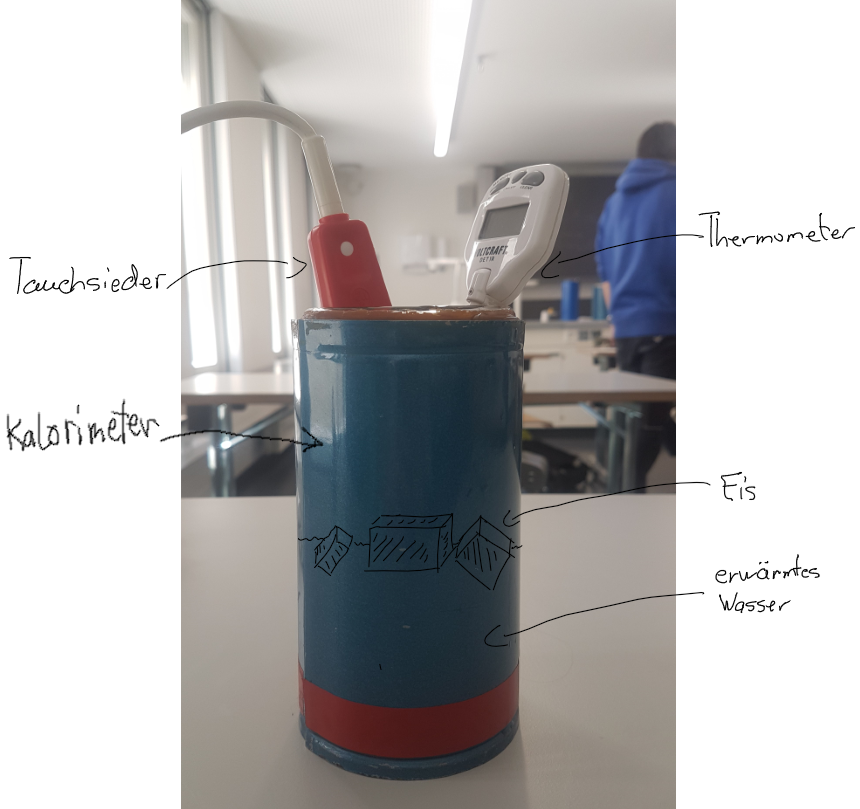
\includegraphics[width=.5\linewidth]{image}
\end{figure}

\section{Versuchsdurchführung}
\begin{table}[H]
    \centering
    \begin{tabular}{|c|c|c|}
        \hline
        \textbf{Beschreibung} & \textbf{Abkürzung} & \textbf{Wert} \\
        \hline
        Wärmekapazität Wasser & $C_{H_{2}O}$ & 4182 $\frac{J}{kg\cdot{}K}$\\
        \hline
        Masse Kalorimeter leer & ${m_{\rm{Kal}}}$ & $(613.0\pm 0.05)g$\\
        Masse Kalorimeter mit Wasser 1 & $m_{1}$ & $(787.0\pm 0.05)g$\\
        \hline
        Masse Gemischt 1 & $m_{2}$ & $(796.9\pm 0.05)g$\\
        Masse Kalorimeter mit Wasser 2 & $m_{3}$ & $(781.3\pm 0.05)g$\\
    Masse Gemischt 2 & $m_{4}$ & $(795.8\pm 0.05)g$\\
        \hline
        Temperatur vor dem Eis 1 & $\vartheta_{T_{1}}$ & $(70.3\pm 0.05)^{\circ}C$\\
        Temperatur geschmolzen 1 & $\vartheta_{T_{2}}$ & $(62.7\pm 0.05) ^{\circ}C$\\
        \hline
        Temperatur vor dem Eis 2 & $\vartheta_{T_{3}}$ & $(63.4\pm 0.05)^{\circ}C$\\
        Temperatur geschmolzen 2 & $\vartheta_{T_{4}}$ & $(54.1\pm 0.05) ^{\circ}C$\\
        \hline
    \end{tabular}
\end{table}
Als erstes wird die Masse des Kalorimeters $m_{\rm{Kal}} $ gemessen  und bis etwa zur Hälfte mit Wasser gefüllt. Die Masse des Kalorimeters mit dem Wasser $m_{\rm{1/3}} $ wird nun nochmals gemessen. Das sich im Kalorimeter befindende Wasser wird mit dem Tauchsieder auf etwa  $\SI{70}{\celsius}$ erwärmt. Die Temperatur des heissen Wassers $\vartheta_{T_{1/3}}$ wird solange gemessen, bis das abgetrocknete Eis ins Wasser hizugegeben wird. Die Temperatur des Wassers wird dann nochmals abgelesen, wenn das Eis sich komplett aufgelöst hat. Die Masse des Kalorimeters mit dem Mischwasser $m_{\rm{2/4}} $ wird nun nochmals gemessen, um die genaue Masse des Eises zu bestimmen.

Die im letzten Paragraphen genannten Schritte werden mit neuem Wasser und neuem Eis wiederholt durchgeführt.
\section{Versuchsauswertung}

$L_{f}= \displaystyle{\frac{m_{\rm{H2O}} \cdot c_{\rm{H_2o}} \cdot \Delta\vartheta_2 - m_{\rm{Eis}} \cdot c_{\rm{H_2O}} \cdot \Delta\vartheta_1}{m_{\rm{Eis}}}}$

\subsection{Durchführung 1}

$L_{f_1}=\displaystyle{\frac{\left(\left(m_1-{m_{\rm{Kal}}}\right) \cdot 4182\rm{\frac{J}{kg \cdot K}}\cdot \left(\vartheta_{T_1}-\vartheta_{T_2}\right)\right)-\left(\left(m_2-m_{1}\right)\cdot 4182 \rm{\frac{J}{kg \cdot K}} \cdot \vartheta_{T_2}\right)}{m_2-{m_{\rm{Kal}}}}} $\\\\

$L_{f_{1_{max}}} =\displaystyle{\frac{\left(0.174\;kg \cdot 4182\rm{\frac{J}{kg \cdot K}}\cdot 7.70^{\circ}C \right)-\left(0.010\;kg\cdot 4182 \rm{\frac{J}{kg \cdot K}} \cdot 62.65^{\circ}C\right)}{0.010\;kg}} = 298302\frac{J}{kg}$\\\\

$L_{f_{1_{min}}} =\displaystyle{\frac{\left(0.174\;kg \cdot 4182\rm{\frac{J}{kg \cdot K}}\cdot 7.50^{\circ}C \right)-\left(0.010\;kg\cdot 4182 \rm{\frac{J}{kg \cdot K}} \cdot 62.75^{\circ}C\right)}{0.010\;kg}} = 283331\frac{J}{kg}$\\\\

$\Rightarrow L_{f_1}=\displaystyle{\frac{L_{1_{max}}+L_{1_{min}}}{2}=\left(290816\pm 7486\right) \cdot \frac{J}{kg}=\left(2.9\pm 0.075\right)\cdot 10^{5} \frac{J}{kg}}$

\subsection{Durchführung 2}

$L_{f_2}=\displaystyle{\frac{\left(\left(m_3-{m_{\rm{Kal}}}\right) \cdot 4182\rm{\frac{J}{kg \cdot K}}\cdot \left(\vartheta_{T_3}-\vartheta_{T_4}\right)\right)-\left(\left(m_4-m_{3}\right)\cdot 4182 \rm{\frac{J}{kg \cdot K}} \cdot \vartheta_{T_3}\right)}{m_4-{m_{\rm{Kal}}}}} $\\\\

$L_{f_{2_{max}}} =\displaystyle{\frac{\left(0.168\;kg \cdot 4182\rm{\frac{J}{kg \cdot K}}\cdot 9.40^{\circ}C \right)-\left(0.015\;kg\cdot 4182 \rm{\frac{J}{kg \cdot K}} \cdot 54.05^{\circ}C\right)}{0.184\;kg}} = 214244\frac{J}{kg}$\\\\

$L_{f_{2_{min}}} =\displaystyle{\frac{\left(0.168\;kg \cdot 4182\rm{\frac{J}{kg \cdot K}}\cdot 9.20^{\circ}C \right)-\left(0.015\;kg\cdot 4182 \rm{\frac{J}{kg \cdot K}} \cdot 54.15^{\circ}C\right)}{0.184\;kg}} = 204458\frac{J}{kg}$\\\\

$\Rightarrow L_{f_2}=\displaystyle{\frac{L_{2_{max}}+L_{2_{min}}}{2}=\left(209351\pm 4893\right) \cdot \frac{J}{kg}=\left(2.1\pm 0.049\right)\cdot 10^{5} \frac{J}{kg}}$

\newpage
\section{Kommentar / Diskussion}

\subsection{Genauigkeit}
Bei den beiden Versuchsdurchgängen wurden beim ersten Mal eine Abweichung von \textit{13\%} und beim zweiten Mal \textit{37\%} festgestellt.\\

Aufgrund der vielen systematischen Fehler, da nicht in einem abgschlossenen System experimentiert werden konnte, kann die Ungenauigkeit der Messresultate erklärt werden. Der Tabellenwert $\num{3.338 e5}\si{\J\per\kg}$ \cite{formelsammlung} wurde wie erwartet unterschritten, da einige Energie aus unserem System an die Umgebung verloren ging.\\

Es ist noch anzumerken, dass bei der Berechnung keine Fehlerschranke bei der Masse gemacht wurde. Dies ist zu begründen, dass diese Ungenauigkeit im Vergleich zur Temperaturmessung vernachlässigbar ist.

\subsection{Fehlerquellen}

Ein systematisch Fehler bestand darin, dass das Kalorimeter nicht zu 100\% isoliert und durch die Wände konstant Energie an die Umwelt abgegeben wird. Vorallem da das Kalorimeter nach oben offen war, entstanden dabei beträchtlich mehr Wärmeverluste am Wasser an die Umgebung als nur den Wänden.\\

Ein weiterer Fehler bestand darin, dass das Eis nicht vollständig mit dem Papier abgetrocknet werden konnte.\\

Beim der zweiten Versuchsdurchführung ist ein kleiner Fehler unterlaufen: Das Eis ist auf den Tisch gefallen und wurde dann mit dem Händen in das Kalorimeter befördert. Dabei ist ein Teil des Eises geschmolzen, weil Wärmeenergie von den Händen an das Eis abgegeben wurde. Somit ist die höhere Abweichung vom Tabellenwert im Vergleich zum ersten Versuchsdurchlauf begründet.

\bibliographystyle{plainnat}
\bibliography{local.bib}

\end{document}
